\documentclass[a4paper, 12pt]{article}
\usepackage{graphicx}
\usepackage{float}
\usepackage{listings}
\usepackage[UTF8]{ctex}
\usepackage{xcolor}
\setlength{\parindent}{2em}
\lstdefinestyle{mybash}{
    language=bash,                 % 设置语言为 Bash[reference:8]
    basicstyle=\small\ttfamily,    % 基础字体：使用等宽字体[reference:9][reference:10]
    keywordstyle=\color{blue},     % 关键字颜色[reference:11][reference:12]
    keywordstyle={[2]\color{cyan}},% 第二组关键字颜色[reference:13]
    commentstyle=\itshape\color{orange!70!black}, % 注释样式：斜体 + 橙色[reference:14]
    stringstyle=\color{teal},      % 字符串颜色[reference:15]
    backgroundcolor=\color{yellow!10}, % 背景色：浅黄色[reference:16][reference:17]
    frame=single,                  % 代码框样式[reference:18]
    numbers=left,                  % 在左侧显示行号[reference:19]
    numberstyle=\tiny\color{gray}, % 行号样式[reference:20]
    breaklines=true,               % 自动换行
    showstringspaces=false,        % 不显示字符串中的空格[reference:21][reference:22]
}
\lstdefinestyle{mypy}{
    language=Python,               % 设置语言为 python[reference:8]
    basicstyle=\small\ttfamily,    % 基础字体：使用等宽字体[reference:9][reference:10]
    keywordstyle=\color{blue},     % 关键字颜色[reference:11][reference:12]
    keywordstyle={[2]\color{cyan}},% 第二组关键字颜色[reference:13]
    commentstyle=\itshape\color{orange!70!black}, % 注释样式：斜体 + 橙色[reference:14]
    stringstyle=\color{teal},      % 字符串颜色[reference:15]
    backgroundcolor=\color{yellow!10}, % 背景色：浅黄色[reference:16][reference:17]
    frame=single,                  % 代码框样式[reference:18]
    numbers=left,                  % 在左侧显示行号[reference:19]
    numberstyle=\tiny\color{gray}, % 行号样式[reference:20]
    breaklines=true,               % 自动换行
    showstringspaces=false,        % 不显示字符串中的空格[reference:21][reference:22]
}

\begin{document}
  \title{Week03 实验报告}
  \author{mrw1114}
  \date{September, 7th}
  \maketitle
  \section{个人信息}
  \begin{itemize}
    \item 姓名：王俊杰
    \item 学号：25020007122
    \item Github 仓库链接：https://github.com/mrw1114/fundamentals-of-system-dev-tools
  \end{itemize}
  \section{课上实验}
    \subsection{第09题：从源码构建并在干净环境安装Wheel}
      \subsubsection{新建相关文件}
      在 q09 中创建好对应的目录结构和文件，并修改为自己的学号。
      \noindent
      \begin{figure}[H]
        \centering
        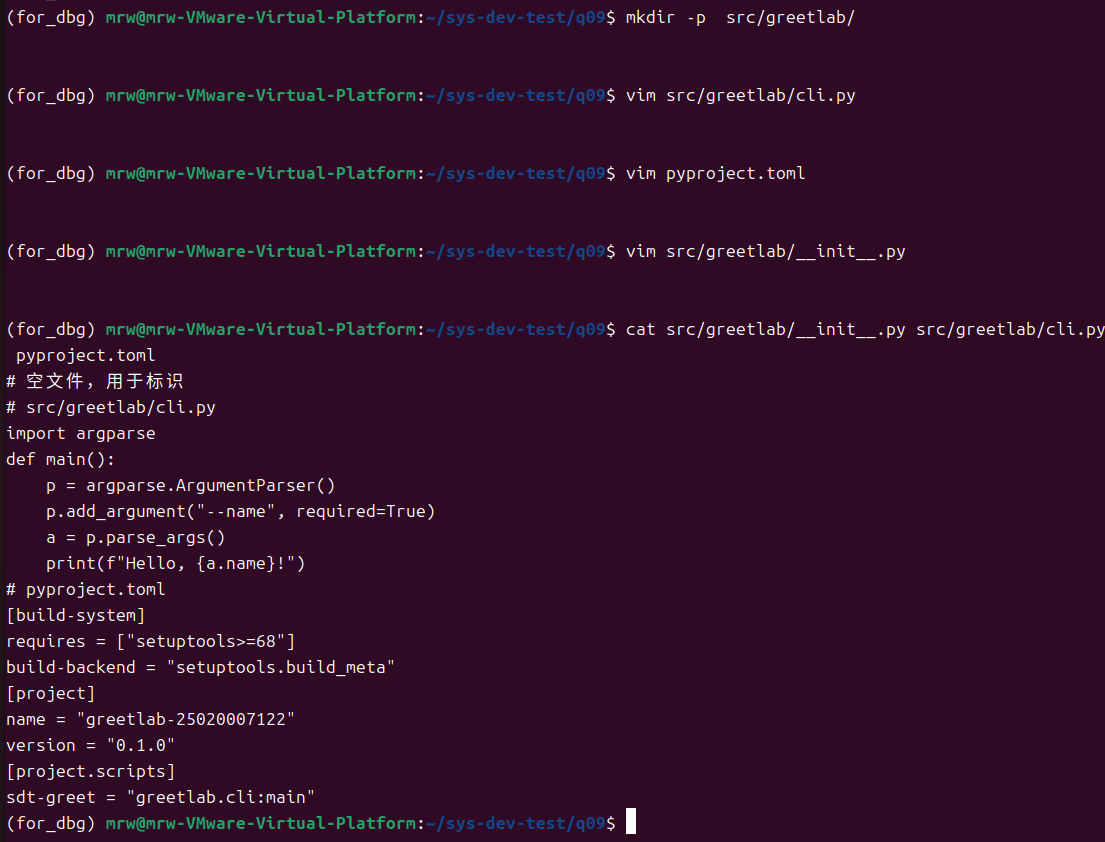
\includegraphics[width=\textwidth]{09-1.png}
        \caption{目录与给定文件的创建}
        \label{09-1}
      \end{figure}
      \subsubsection{使用 build 构建 whell}
      在已经安装好 build 包的 for\_dbg 环境中执行 python -m build . 从当前目录构建 greetlab\_25020007122。构建好的 wheel 文件位于当前目录的 dist 文件夹中。
      \noindent
      \begin{figure}[H]
        \centering
        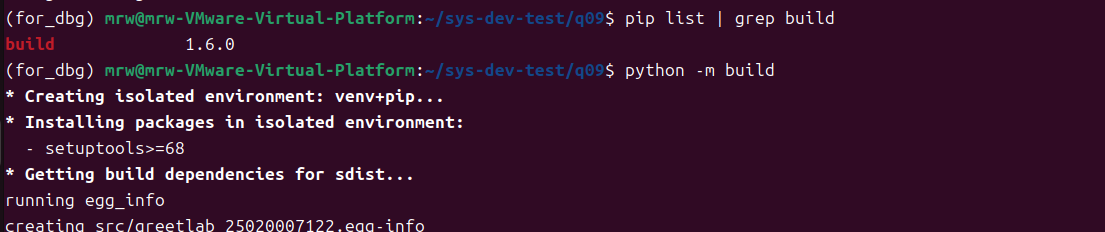
\includegraphics[width=\textwidth]{09-2-1.png}
        \caption{在 for\_dbg 中执行构建命令}
        \label{09-2-1}
      \end{figure}
      \noindent
      \begin{figure}[H]
        \centering
        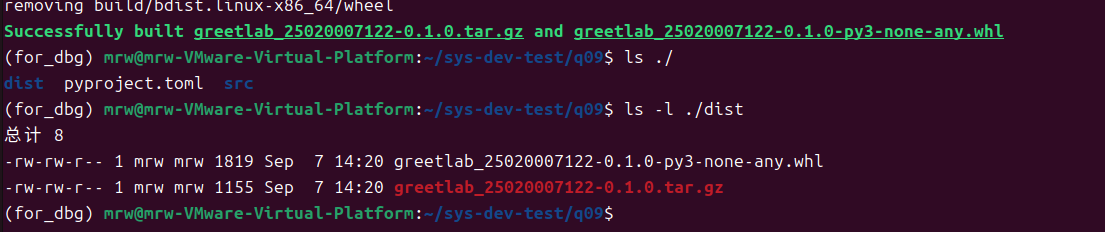
\includegraphics[width=\textwidth]{09-2-2.png}
        \caption{执行后的构建产物}
        \label{09-2-2}
      \end{figure}
      \subsubsection{切换虚拟环境并安装 wheel}
      禁用 for\_dbg 环境，使用 python3 -m venv venv 在 q09 下新建虚拟环境 venv；使用 source venv/bin/activate 启用虚拟环境；随后使用 pip install dist/greetlab\_25020007122-0.1.0-py3-none-any.whl 安装构建的包。
      \noindent
      \begin{figure}[H]
        \centering
        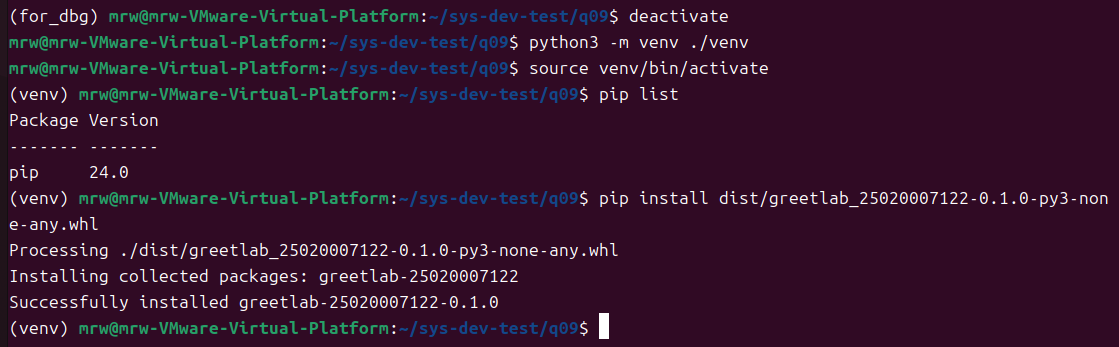
\includegraphics[width=\textwidth]{09-3.png}
        \caption{虚拟环境的构建与包的安装}
        \label{09-3}
      \end{figure}
      \subsubsection{测试是否成功安装}
      切换到上级目录，执行 sdt-greet \detokenize{--}name 25020007122 可以确认构建的包已成功安装。
      \noindent
      \begin{figure}[H]
        \centering
        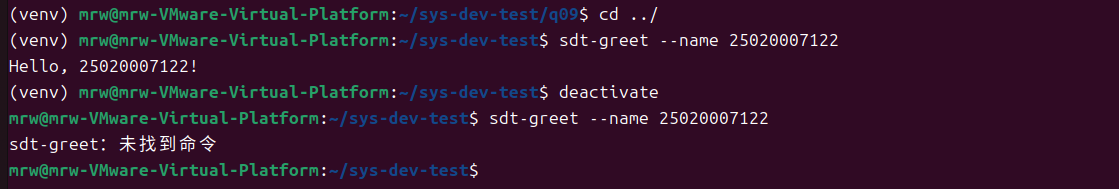
\includegraphics[width=\textwidth]{09-4.png}
        \caption{命令执行结果}
        \label{09-4}
      \end{figure}
    \subsection{第10题：让编程智能体进入可验证的修复循环}
    \noindent
    由于虚拟机环境限制，此处通过虚拟文件夹等方式将 q09 中的相关文件复制到 Windows 系统上进行，使用 TRAE 作为编程所需的智能体。
      \subsubsection{新建 pytest 测试}
      在 Windows 平台上重新进行构建和安装。随后在 q10 下新建 test/test\_cli.py 测试执行 sdt-greet \detokenize{--}name “    ” 时是否报错并返回2，结果发现测试不通过，命令执行并返回0
      \noindent
      \begin{figure}[H]
        \centering
        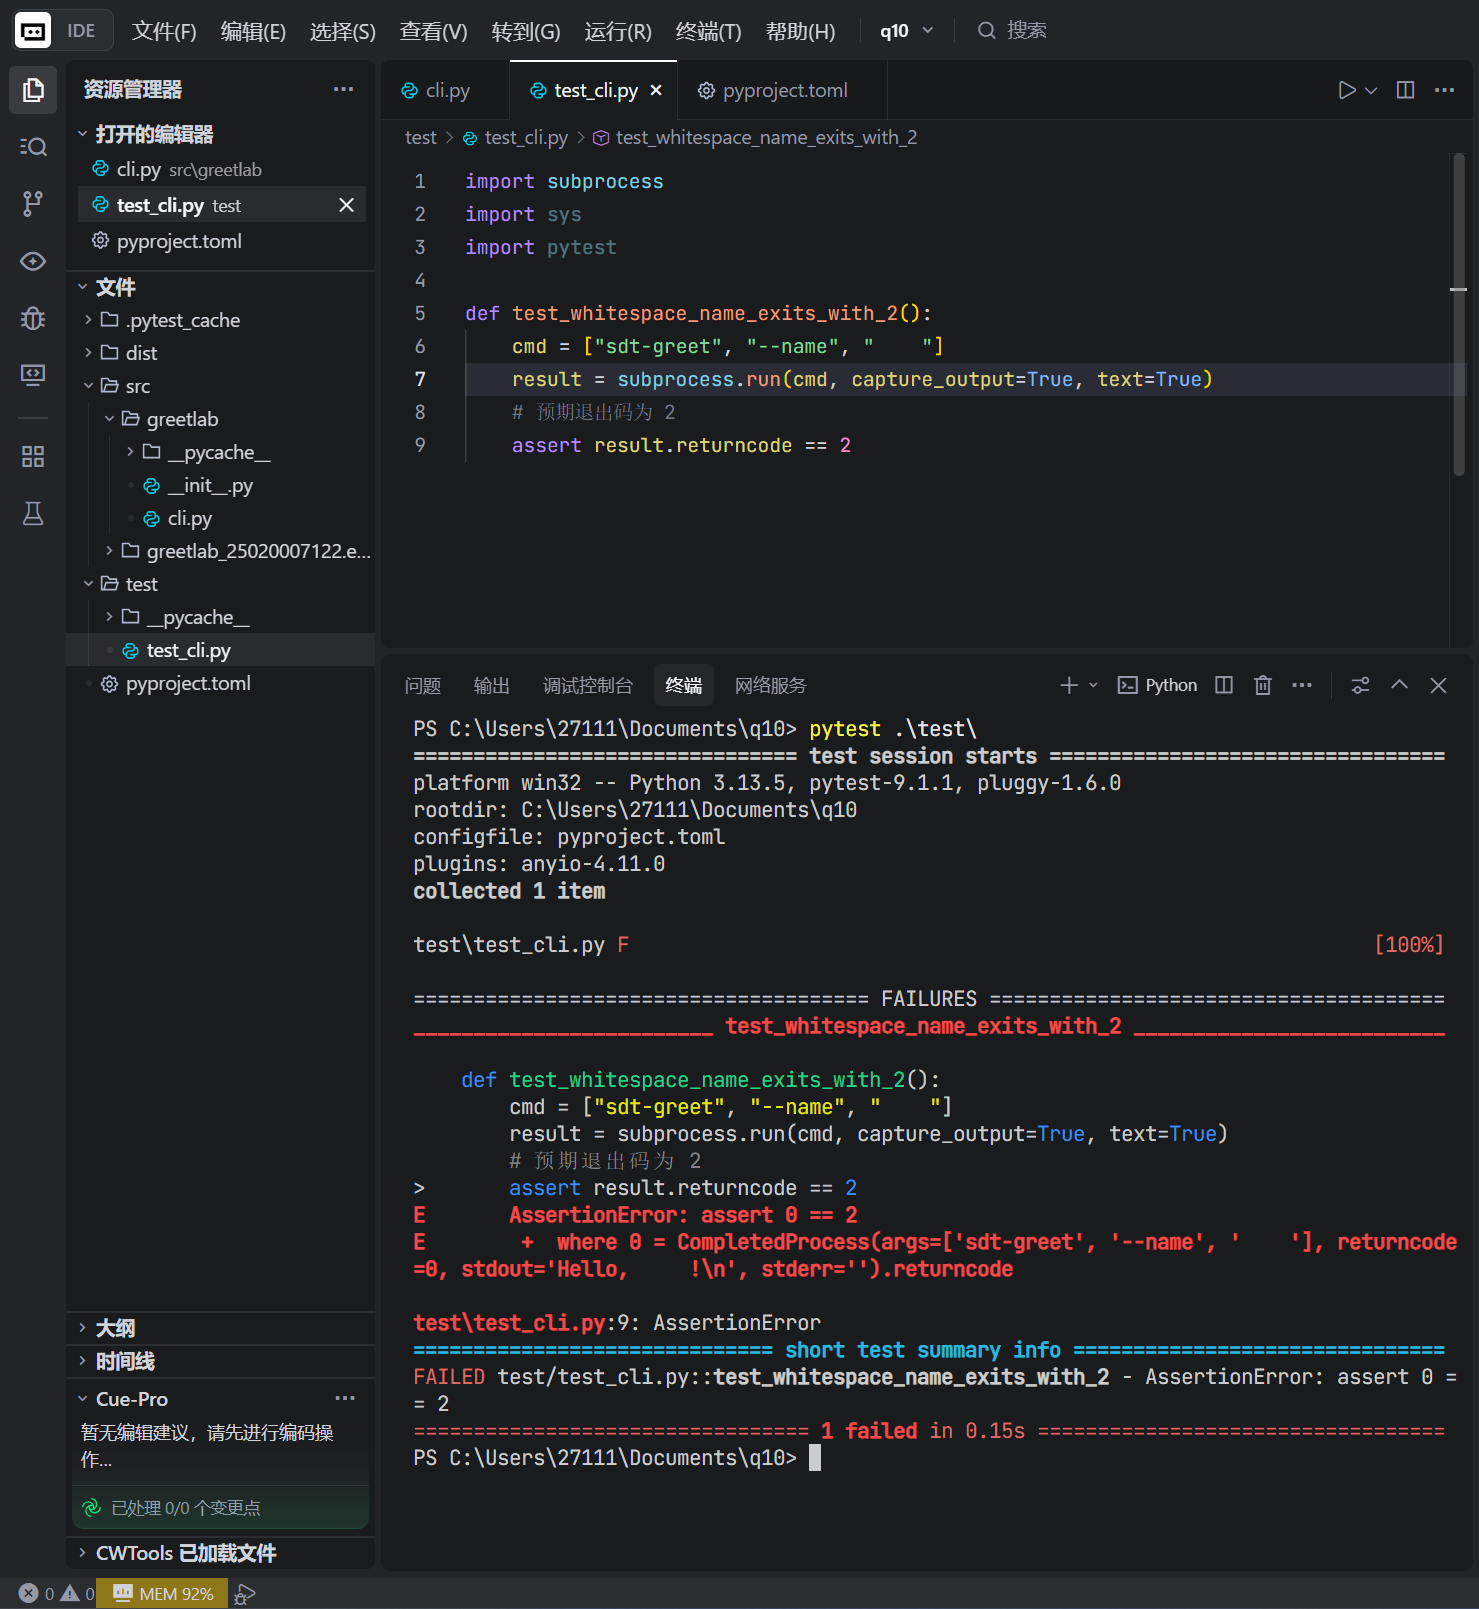
\includegraphics[width=\textwidth]{10-1.png}
        \caption{第一次测试结果}
        \label{10-1}
      \end{figure}
      \subsubsection{向 Agent 发出指令并等待其修复完成}
      向 Agent 发送命令，指定其在 src/greetlab/cli.py 中修复该问题并修改 pyproject.toml 中的版本号；完成修复后，自行构建 wheel 并安装，再使用 pytest 进行测试。等待 Agent 完成命令。
      \noindent
      \begin{figure}[H]
        \centering
        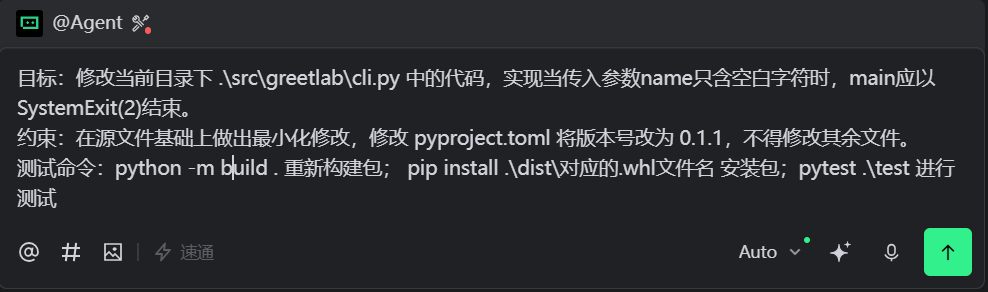
\includegraphics[width=\textwidth]{10-2-1.png}
        \caption{向 Agent 发送的提示词}
        \label{10-2-1}
      \end{figure}
      \noindent
      \begin{figure}[H]
        \centering
        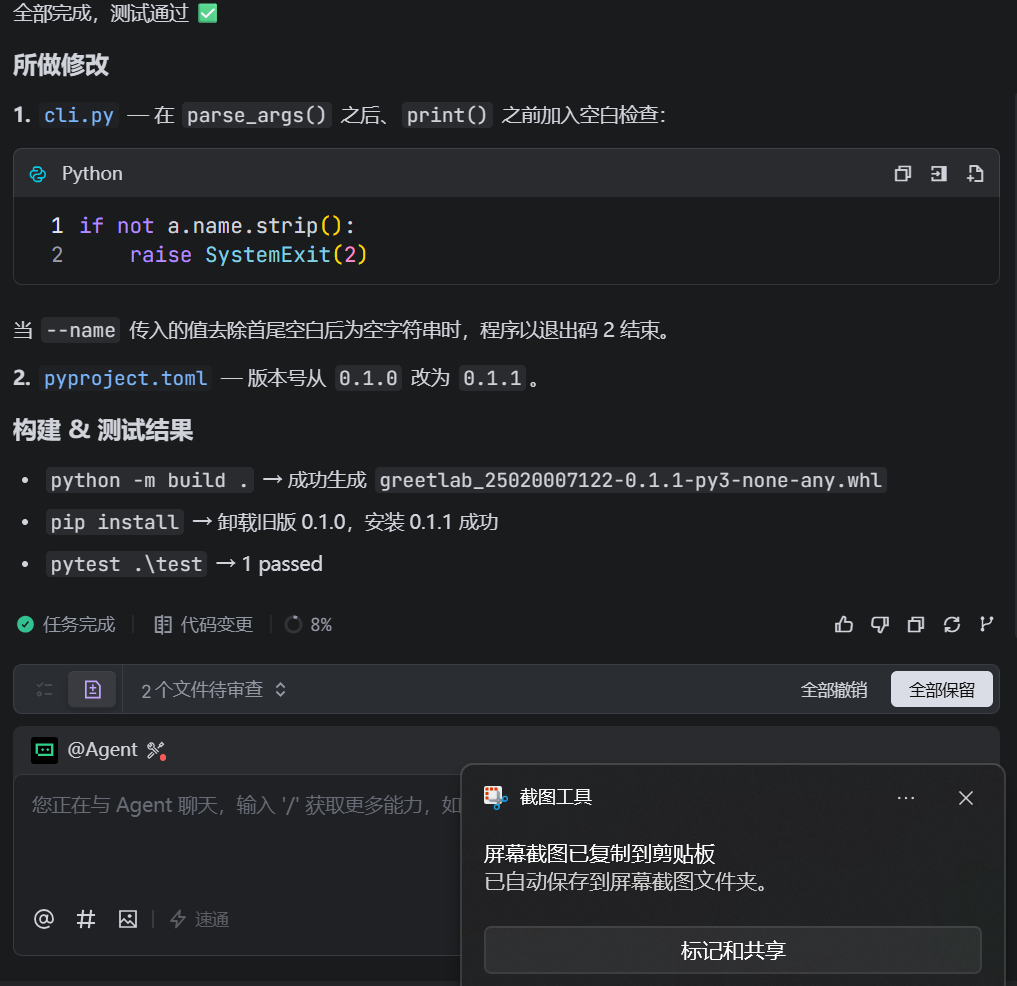
\includegraphics[width=\textwidth]{10-2-2.png}
        \caption{Agent 的执行结果}
        \label{10-2-2}
      \end{figure}
      \subsubsection{对 diff 进行审批}
      查看发生变动的两个文件的差异，均可接受。
      \noindent
      \begin{figure}[H]
        \centering
        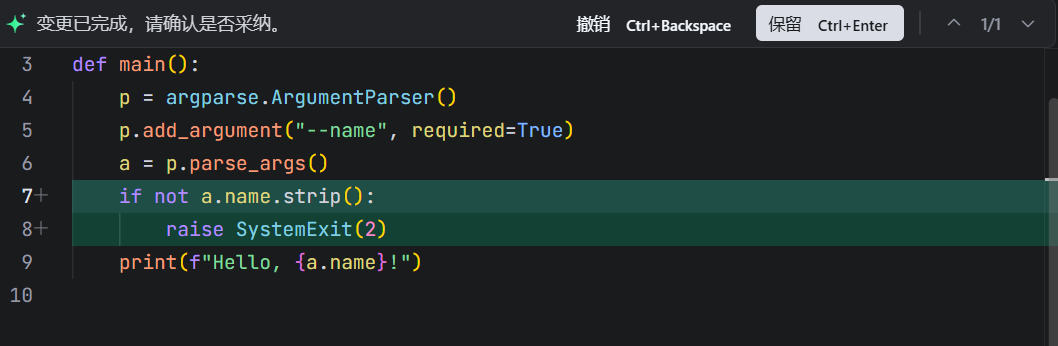
\includegraphics[width=\textwidth]{10-3-1.png}
        \caption{src/greetlab/cli.py 的 diff}
        \label{10-3-1}
      \end{figure}
      \noindent
      \begin{figure}[H]
        \centering
        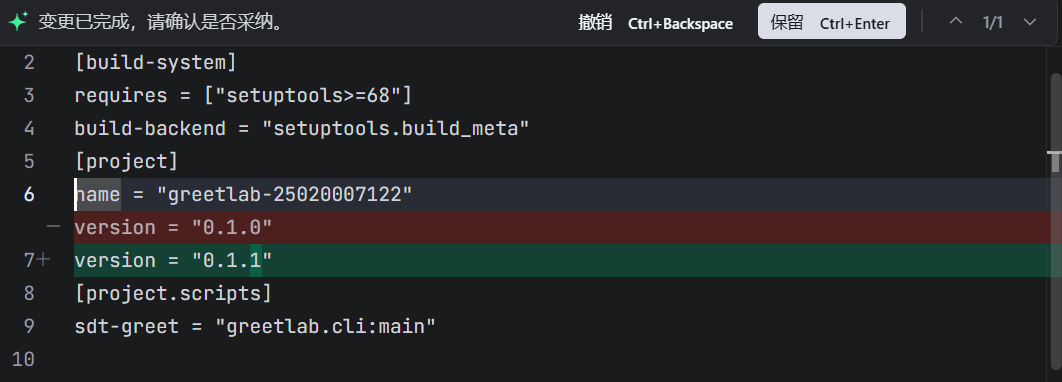
\includegraphics[width=\textwidth]{10-3-2.png}
        \caption{pyproject.toml 的 diff}
        \label{10-3-2}
      \end{figure}
      \subsubsection{新建 pytest 测试}
      审批完成后，手动进行 wheel 的构建和安装，进行 pytest 发现测试通过。
      \noindent
      \begin{figure}[H]
        \centering
        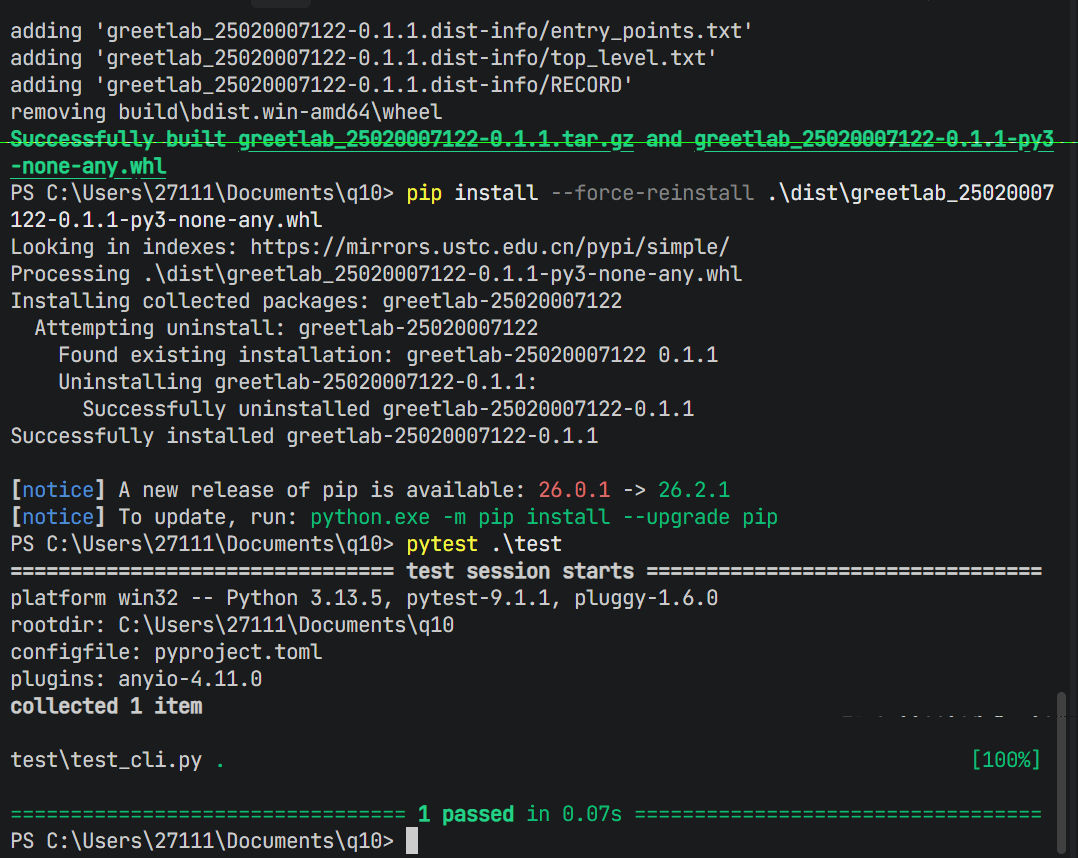
\includegraphics[width=\textwidth]{10-4.png}
        \caption{第二次测试结果}
        \label{10-4}
      \end{figure}
      \subsubsection{记录智能体维护行为到 ai\_log.md中}
      将核心提示、智能体改动、人工验证等信息记录到 ai\_log.md 中并保存。
      \noindent
      \begin{figure}[H]
        \centering
        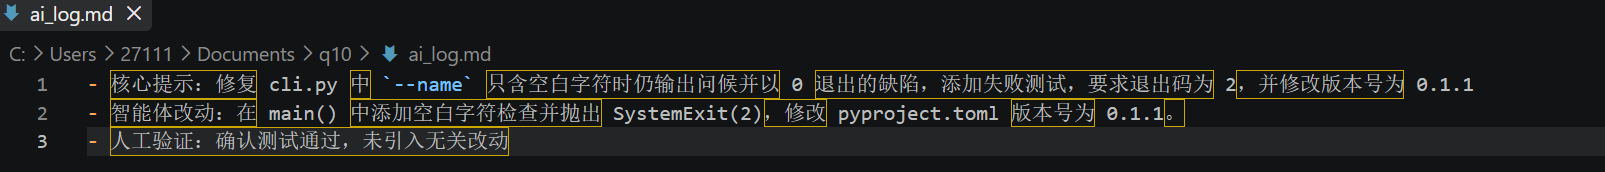
\includegraphics[width=\textwidth]{10-5.png}
        \caption{ai\_log.md 内容}
        \label{10-5}
      \end{figure}
    \subsection{第11题：把“无法处理”的协作材料改成可执行信息}
      \subsubsection{完善沟通信息}
      根据题目要求完善相关信息，补全对应的上下文。此处 Blocking、Suggestion 或 Nit 表征代码审查中得到问题的严重程度，分别表示：导致程序无法正常运行的重大缺陷（功能缺失、逻辑错误、安全漏洞等）、可供优化的功能问题、代码风格等小瑕疵。
      \noindent
      \begin{figure}[H]
        \centering
        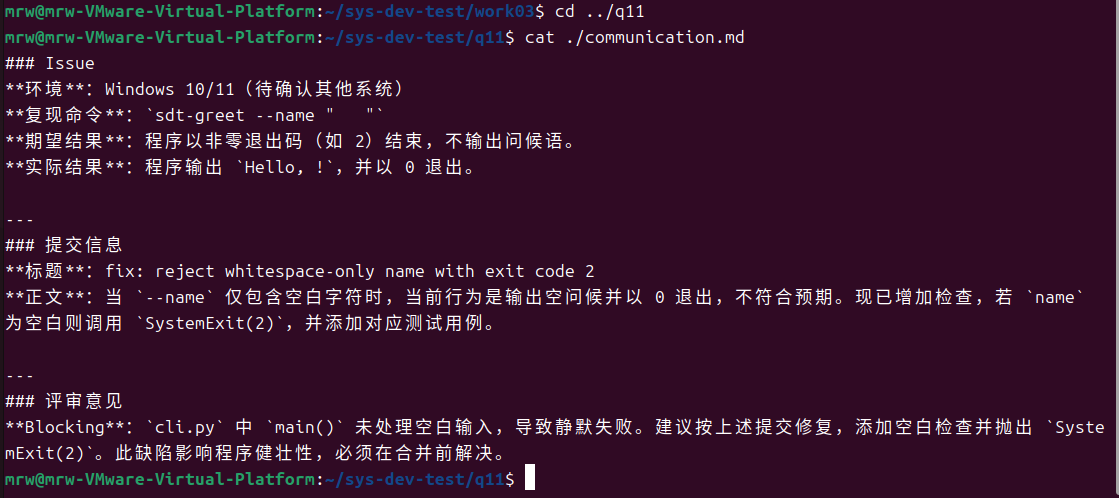
\includegraphics[width=\textwidth]{11.png}
        \caption{编辑完成的 communication.md 文件}
        \label{11}
      \end{figure}
    \subsection{第12题：修复一个可复现的线性回归训练循环}
      \subsubsection{新建相关文件并完善相应的环境}
      在 q12 下新建 train.py 文件，随后新建 for\_pytorch 环境并且在环境中安装 pytorch（需要选择 torch 作为安装的包名）。
      \noindent
      \begin{figure}[H]
        \centering
        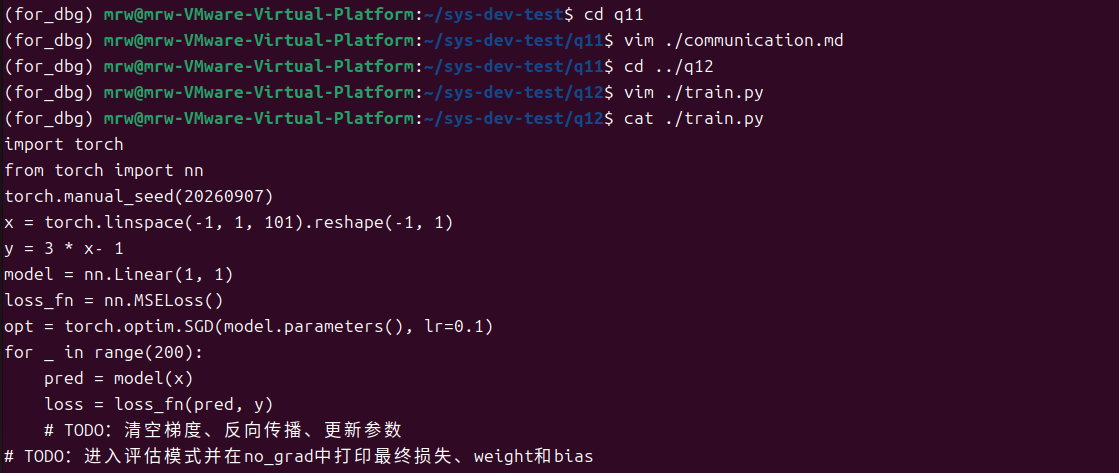
\includegraphics[width=\textwidth]{12-1-1.png}
        \caption{新建给定的 train.py 文件}
        \label{12-1-1}
      \end{figure}
      \noindent
      \begin{figure}[H]
        \centering
        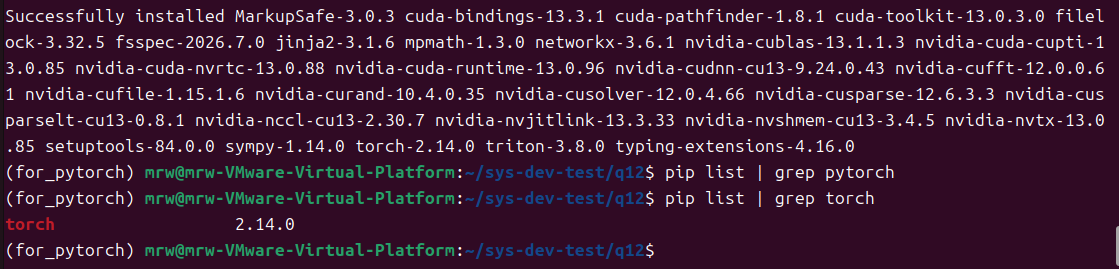
\includegraphics[width=\textwidth]{12-1-2.png}
        \caption{配置虚拟环境}
        \label{12-1-2}
      \end{figure}
\subsubsection{新建相关文件并完善相应的环境}
      根据提示和注释完善 trian.py
\begin{lstlisting}[caption={完善后的 train.py},style=mypy]
import torch
from torch import nn
torch.manual_seed(20260907)
x = torch.linspace(-1, 1, 101).reshape(-1, 1)
y = 3 * x - 1
model = nn.Linear(1, 1)
loss_fn = nn.MSELoss()
opt = torch.optim.SGD(model.parameters(), lr=0.1)
for _ in range(200):
    pred = model(x)
    loss = loss_fn(pred, y)
    # TODO：清空梯度、反向传播、更新参数
    opt.zero_grad()
    loss.backward()
    opt.step()
# TODO：进入评估模式并在 no_grad 中打印最终损失、weight 和 bias
model.eval()
with torch.no_grad():
    final_pred = model(x)
    final_loss = loss_fn(final_pred, y)
    weight = model.weight.item()
    bias = model.bias.item()
    print(f"Final loss: {final_loss:.6f}")
    print(f"weight: {weight:.6f}, bias: {bias:.6f}")
\end{lstlisting}
      \subsubsection{查看训练结果}
      运行 train.py 观察模型拟合结果。
      \noindent
      \begin{figure}[H]
        \centering
        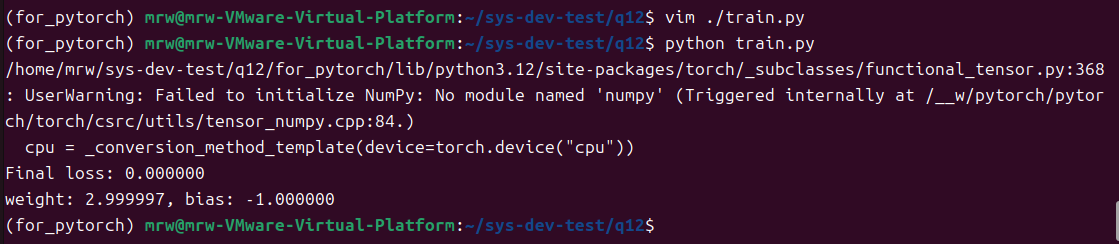
\includegraphics[width=\textwidth]{12-3.png}
        \caption{模型拟合结果}
        \label{12-3}
      \end{figure}
  \section{课后练习}
    \subsection{第01题}
      \subsubsection{题目描述}
      Save your environment with printenv to a file, create a venv, activate it, printenv to another file, and diff before.txt after.txt. What changed in the environment? Why does the shell prefer the venv? (Hint: look at \$PATH before and after activation.) Run which deactivate and reason about what the deactivate bash function is doing.（将你的环境用 printenv 保存到文件，创建虚拟环境，激活它，再用 printenv 保存到另一个文件，并 diff before.txt after.txt。环境发生了什么变化？为什么 shell 优先使用虚拟环境？（提示：查看激活前后的 \$PATH。）运行 which deactivate，并推理 deactivate bash 函数在做什么。）
      \subsubsection{解题过程}
      先在未激活任何虚拟环境的终端中，保存当前环境变量到 before.txt ，随后用 python -m venv test 在当前目录创建一个虚拟环境 test，并用 source 命令加载 test/bin/activate 中的定义到终端中从而激活虚拟环境，保存环境变量到 after.txt 中再用 diff 比较两个文件差异。可以发现环境变量中新增了变量 VIRTUAL\_ENV 指向当前激活的虚拟环境所在目录，以及 VIRTUAL\_ENV\_PROMPT 用作提示，原有的 PS1 变量在前面加入了 VIRTUAL\_ENV\_PROMPT 的内容用作命令提示符内容的更新, PATH 变量则加入了虚拟环境 bin 目录指定可执行文件查找地址。执行 type deactivate 来查看其定义，发现这个函数执行时会复原 PATH，PYTHONHOME，PS1，并最后清除新引入的变量和自己。
      \noindent
      \begin{figure}[H]
        \centering
        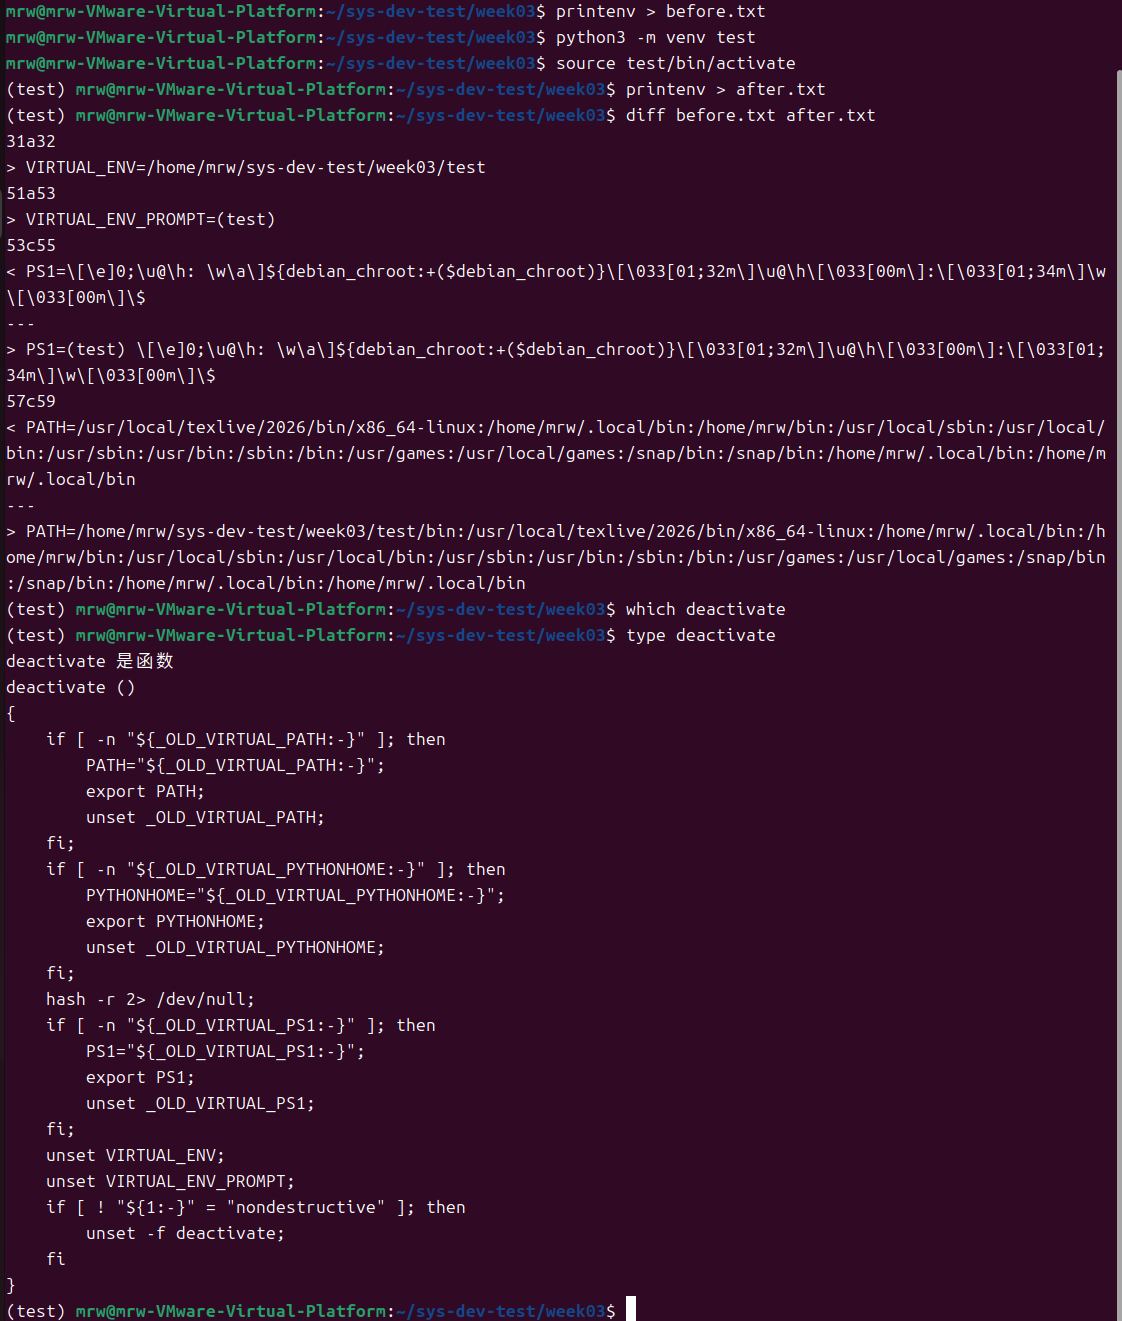
\includegraphics[width=\textwidth]{work03-1.png}
        \caption{虚拟环境激活前后环境变量的比较与 deactivate 函数的定义}
        \label{work03-1}
      \end{figure}
    \subsection{第02题}
      \subsubsection{题目描述}
      Install Docker and use it to build the Missing Semester class website locally using docker compose.（安装 Docker，并使用 docker compose 在本地构建 Missing Semester 课程网站。）
      \subsubsection{解题过程}
      （由于网络原因需要在容器内设置 apk 换源）首先使用 git clone 获取课程仓库，进入仓库所在路径，检查发现存在 docker-compose.yml 与 Dockerfile。由于 Dockerfile 没有进行 apk 换源会导致容器构建缓慢，故修改 Dockerfile 使之使用国内镜像源。接下来执行 sudo docker compose up -d 构建容器在后台运行，随后根据其中内容访问开放在本地 4000 端口的服务。
      \noindent
      \begin{figure}[H]
        \centering
        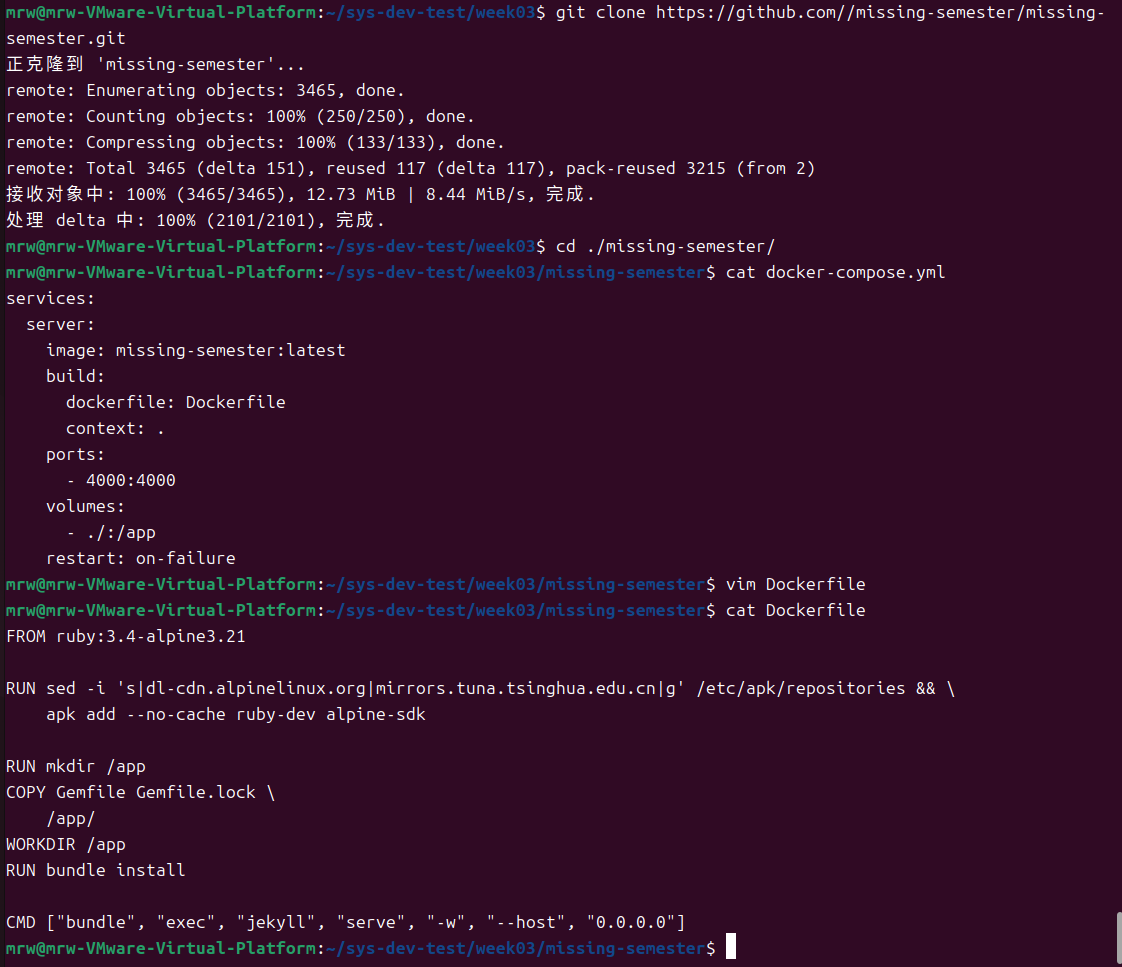
\includegraphics[width=\textwidth]{work03-2-1.png}
        \caption{课程网站仓库克隆与 Dockerfile 修改}
        \label{work03-2-1}
      \end{figure}
      \noindent
      \begin{figure}[H]
        \centering
        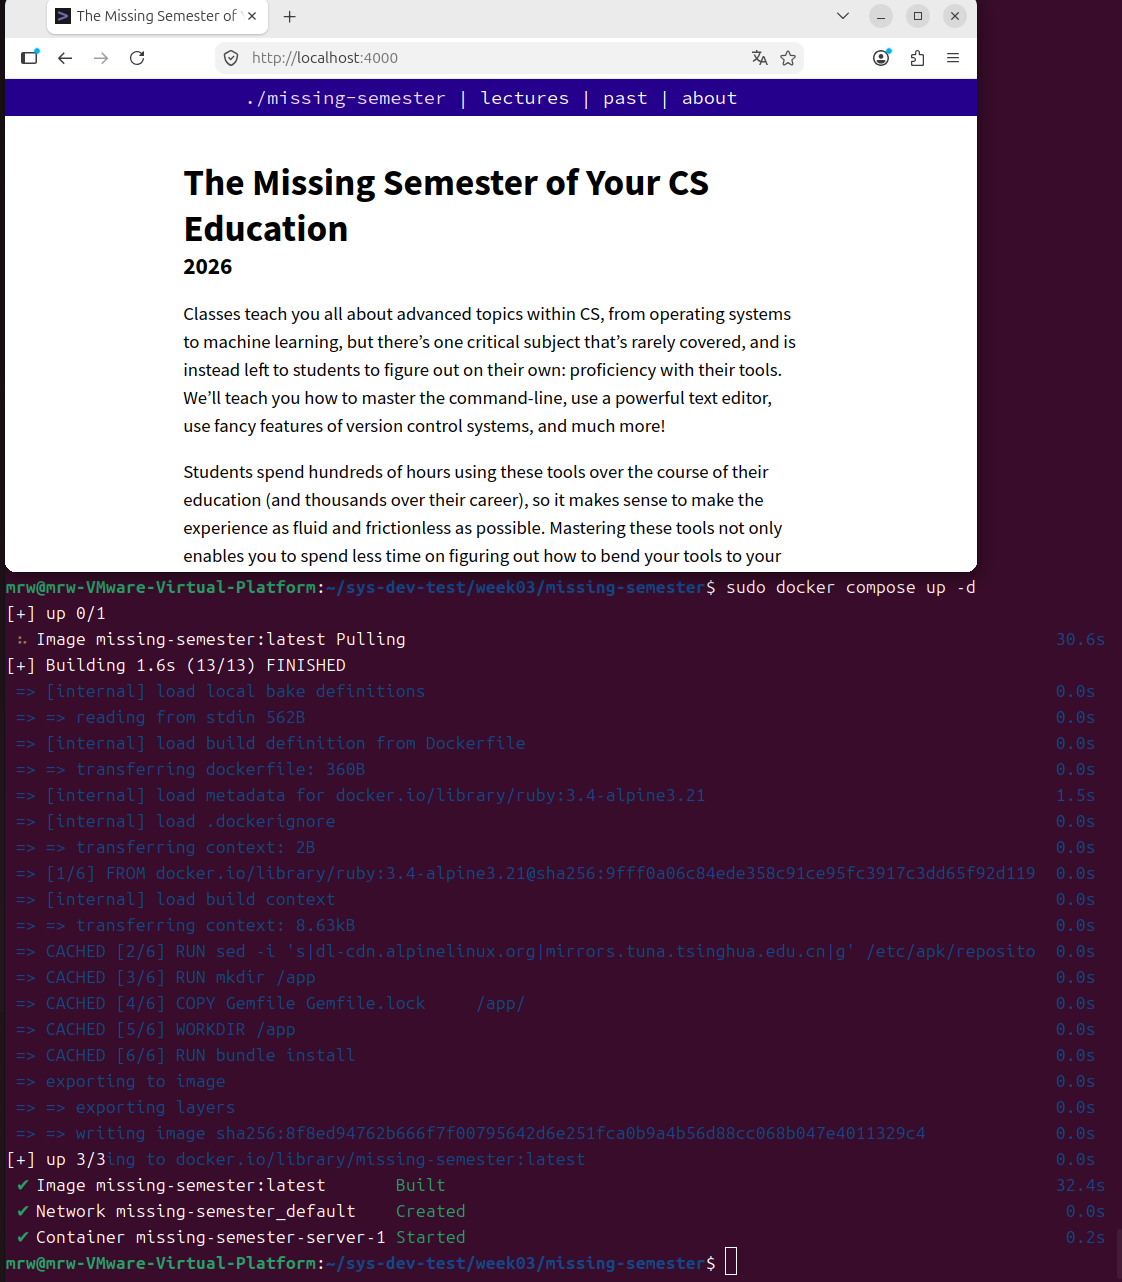
\includegraphics[width=\textwidth]{work03-2-2.png}
        \caption{课程网站的构建与访问} 
        \label{work03-2-2}
      \end{figure}
    \subsection{第03题}
      \subsubsection{题目描述}
      Write a Dockerfile for a simple Python application. Then write a docker-compose.yml that runs your application alongside a Redis cache.（为一个简单的 Python 应用编写 Dockerfile。然后编写 docker-compose.yml，让应用与 Redis 缓存一起运行。）
      \subsubsection{解题过程}
      创建相关数据文件，随后运行 docker-compose up --build 启动服务器。
      \noindent
      \begin{figure}[H]
        \centering
        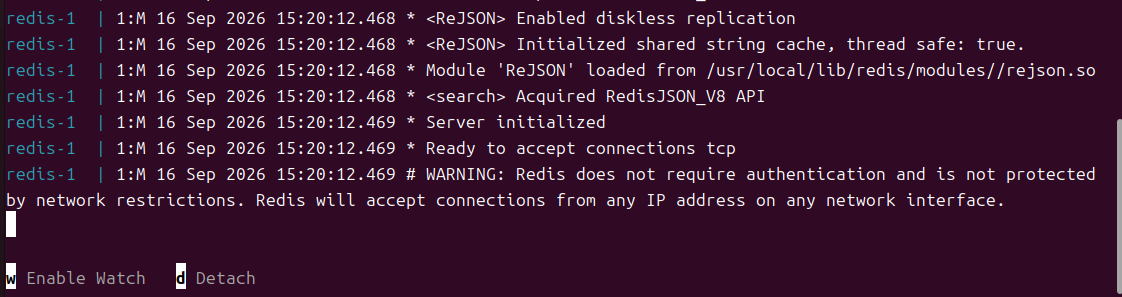
\includegraphics[width=\textwidth]{work03-3-2.png}
        \caption{搭建效果}
        \label{work03-3-2}
      \end{figure}
    \subsection{第04题}
      \subsubsection{题目描述}
      Create a Python package with a pyproject.toml and install it in a virtual environment. Create a lockfile and inspect it.（创建一个带有 pyproject.toml 的 Python 包，并在虚拟环境中安装它。创建一个锁文件并检查它。）
      \subsubsection{解题过程}
      使用 q10 中的 greetlab 包，将其复制到工作目录中，进入该目录。由于虚拟环境的路径问题，需要删除原有的 venv 虚拟环境再生成一个 venv 虚拟环境，随后激活虚拟环境，安装并更新 pip-tools
      \noindent
      \begin{figure}[H]
        \centering
        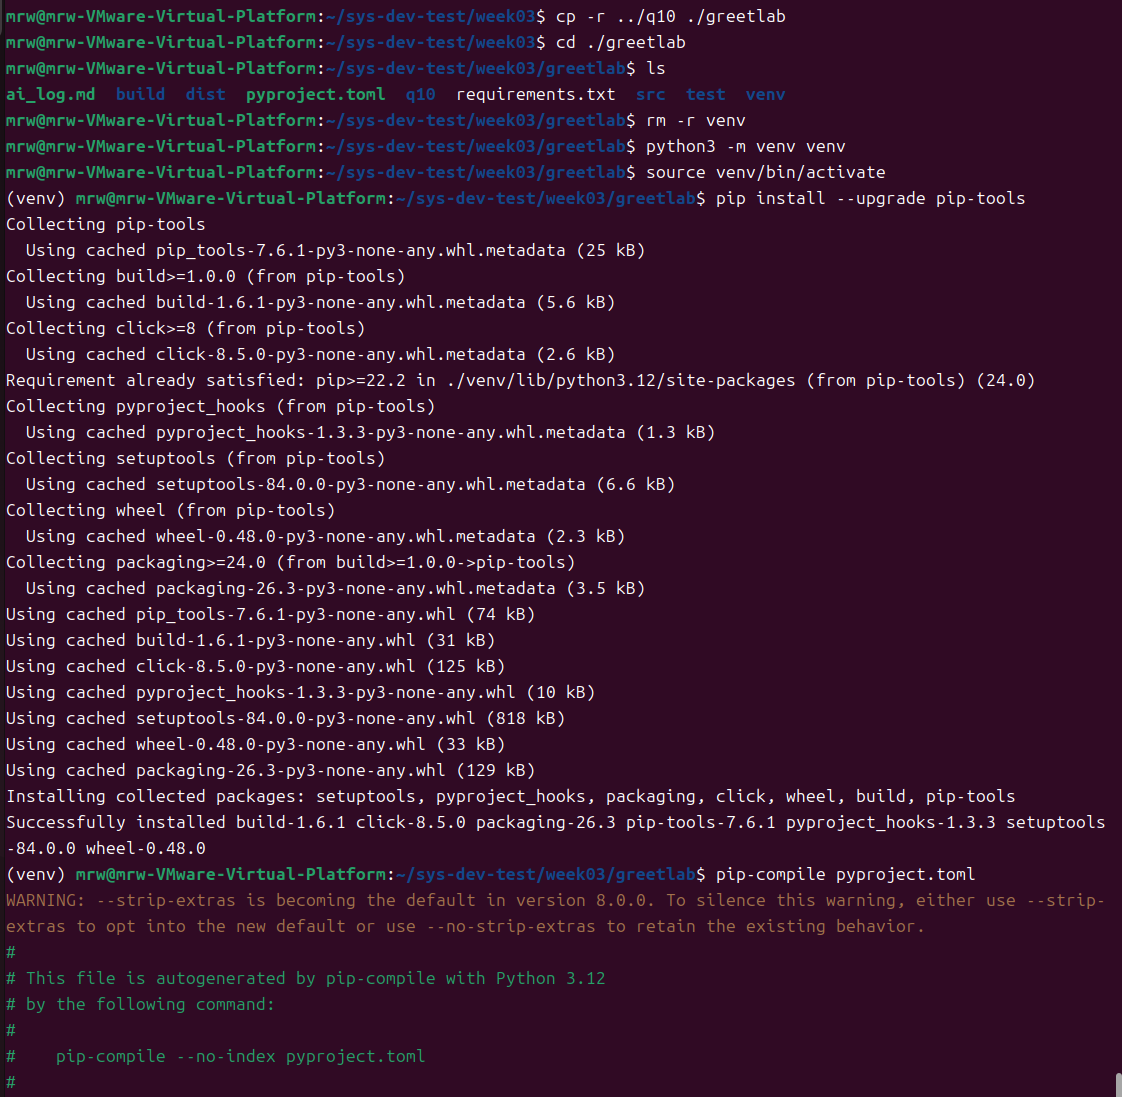
\includegraphics[width=\textwidth]{work03-4-1}
        \caption{创建虚拟环境并制造锁文件} 
        \label{work03-4-1}
      \end{figure}
      \noindent
      \begin{figure}[H]
        \centering
        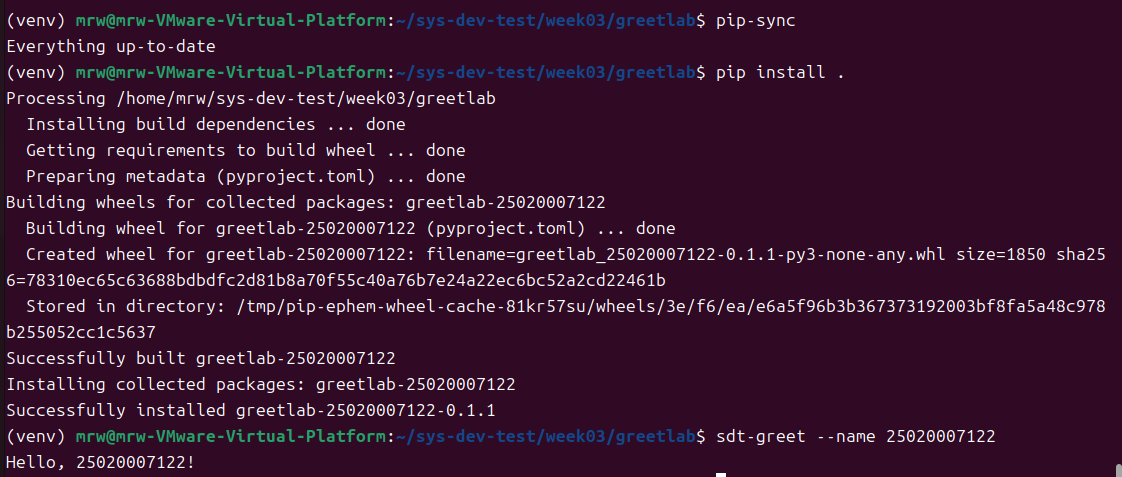
\includegraphics[width=\textwidth]{work03-4-2}
        \caption{同步依赖并安装 python 包}
        \label{work03-4-2}
      \end{figure}
    \subsection{第05题}
      \subsubsection{题目描述}
      浏览一个知名项目（例如 Redis 或 curl）的源码。找出讲义中提到的几种注释类型：有用的 TODO、指向外部文档的引用、解释为何避开某种做法的“why not”注释、或血泪教训。如果这些注释不存在，会失去什么？
      \subsubsection{解题过程}
      获取 redis 的源码仓库并使用 grep 查看相关注释，若这些注释不存在将导致维护时缺少上下文信息，增加不必要的麻烦和制造出 bug 的潜在风险
      \noindent
      \begin{figure}[H]
        \centering
        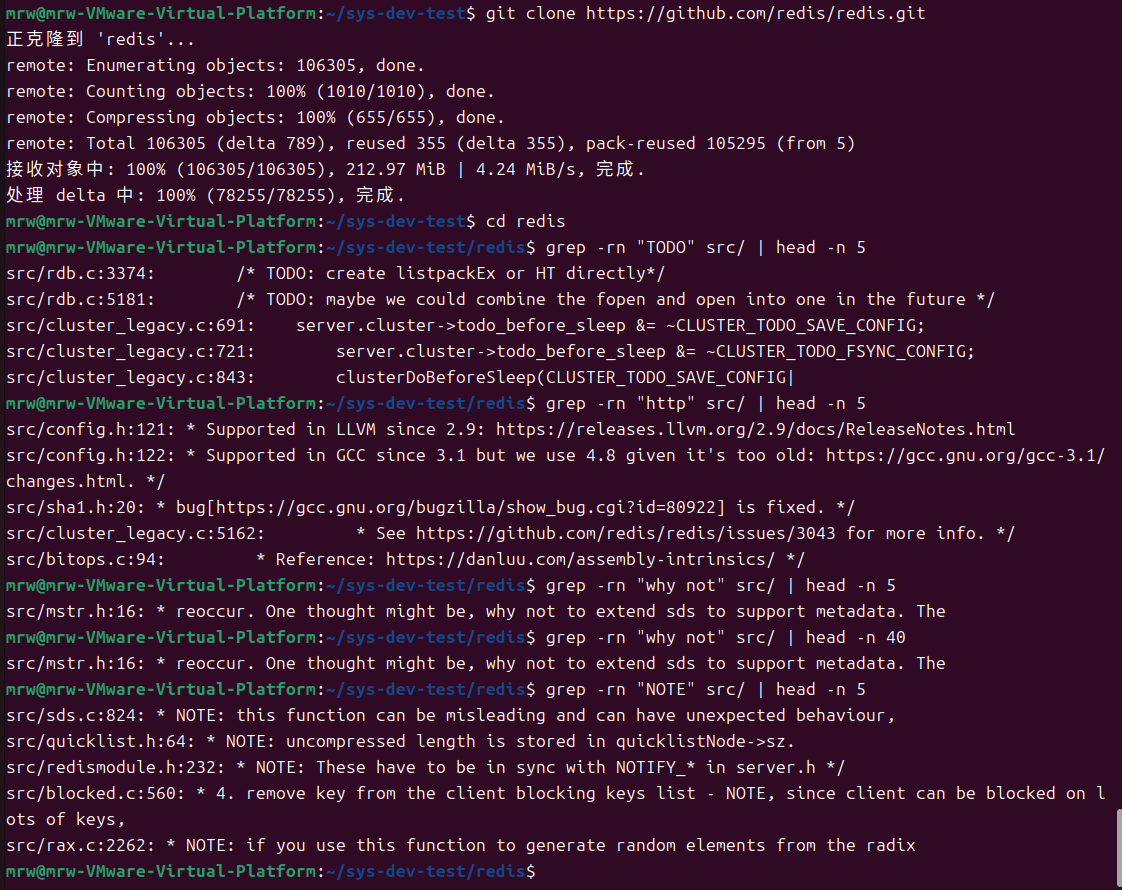
\includegraphics[width=\textwidth]{work03-5.png}
        \caption{获取 redis 的源码并查看相关注释} 
        \label{work03-5}
      \end{figure}
    \subsection{第06题}
      \subsubsection{题目描述}
      对比三个 1000+ star 的 GitHub 项目的 README。它们都同样有用吗？找出哪些内容在你看来主要是噪音，为你将来写 README 提供借鉴。
      \subsubsection{解题过程}
      对kubernetes-client/java、GZCTF、move-language/move 的三个仓库的 README 进行分析：kubernetes-client/java 结构完善，清晰区分了安装、版本兼容、开发与支持入口。GZCTF 极简，开篇引导至外部文档，目标导向性强。move-language/move 告知项目已停更并指引新仓库。三者均无明显噪音，都没把完整文档塞进 README。这说明写 README 时应直接说明项目定位与状态，使用必要的链接引用，保持精炼并针对用户的不同需求设计。
      \noindent
      \begin{figure}[H]
        \centering
        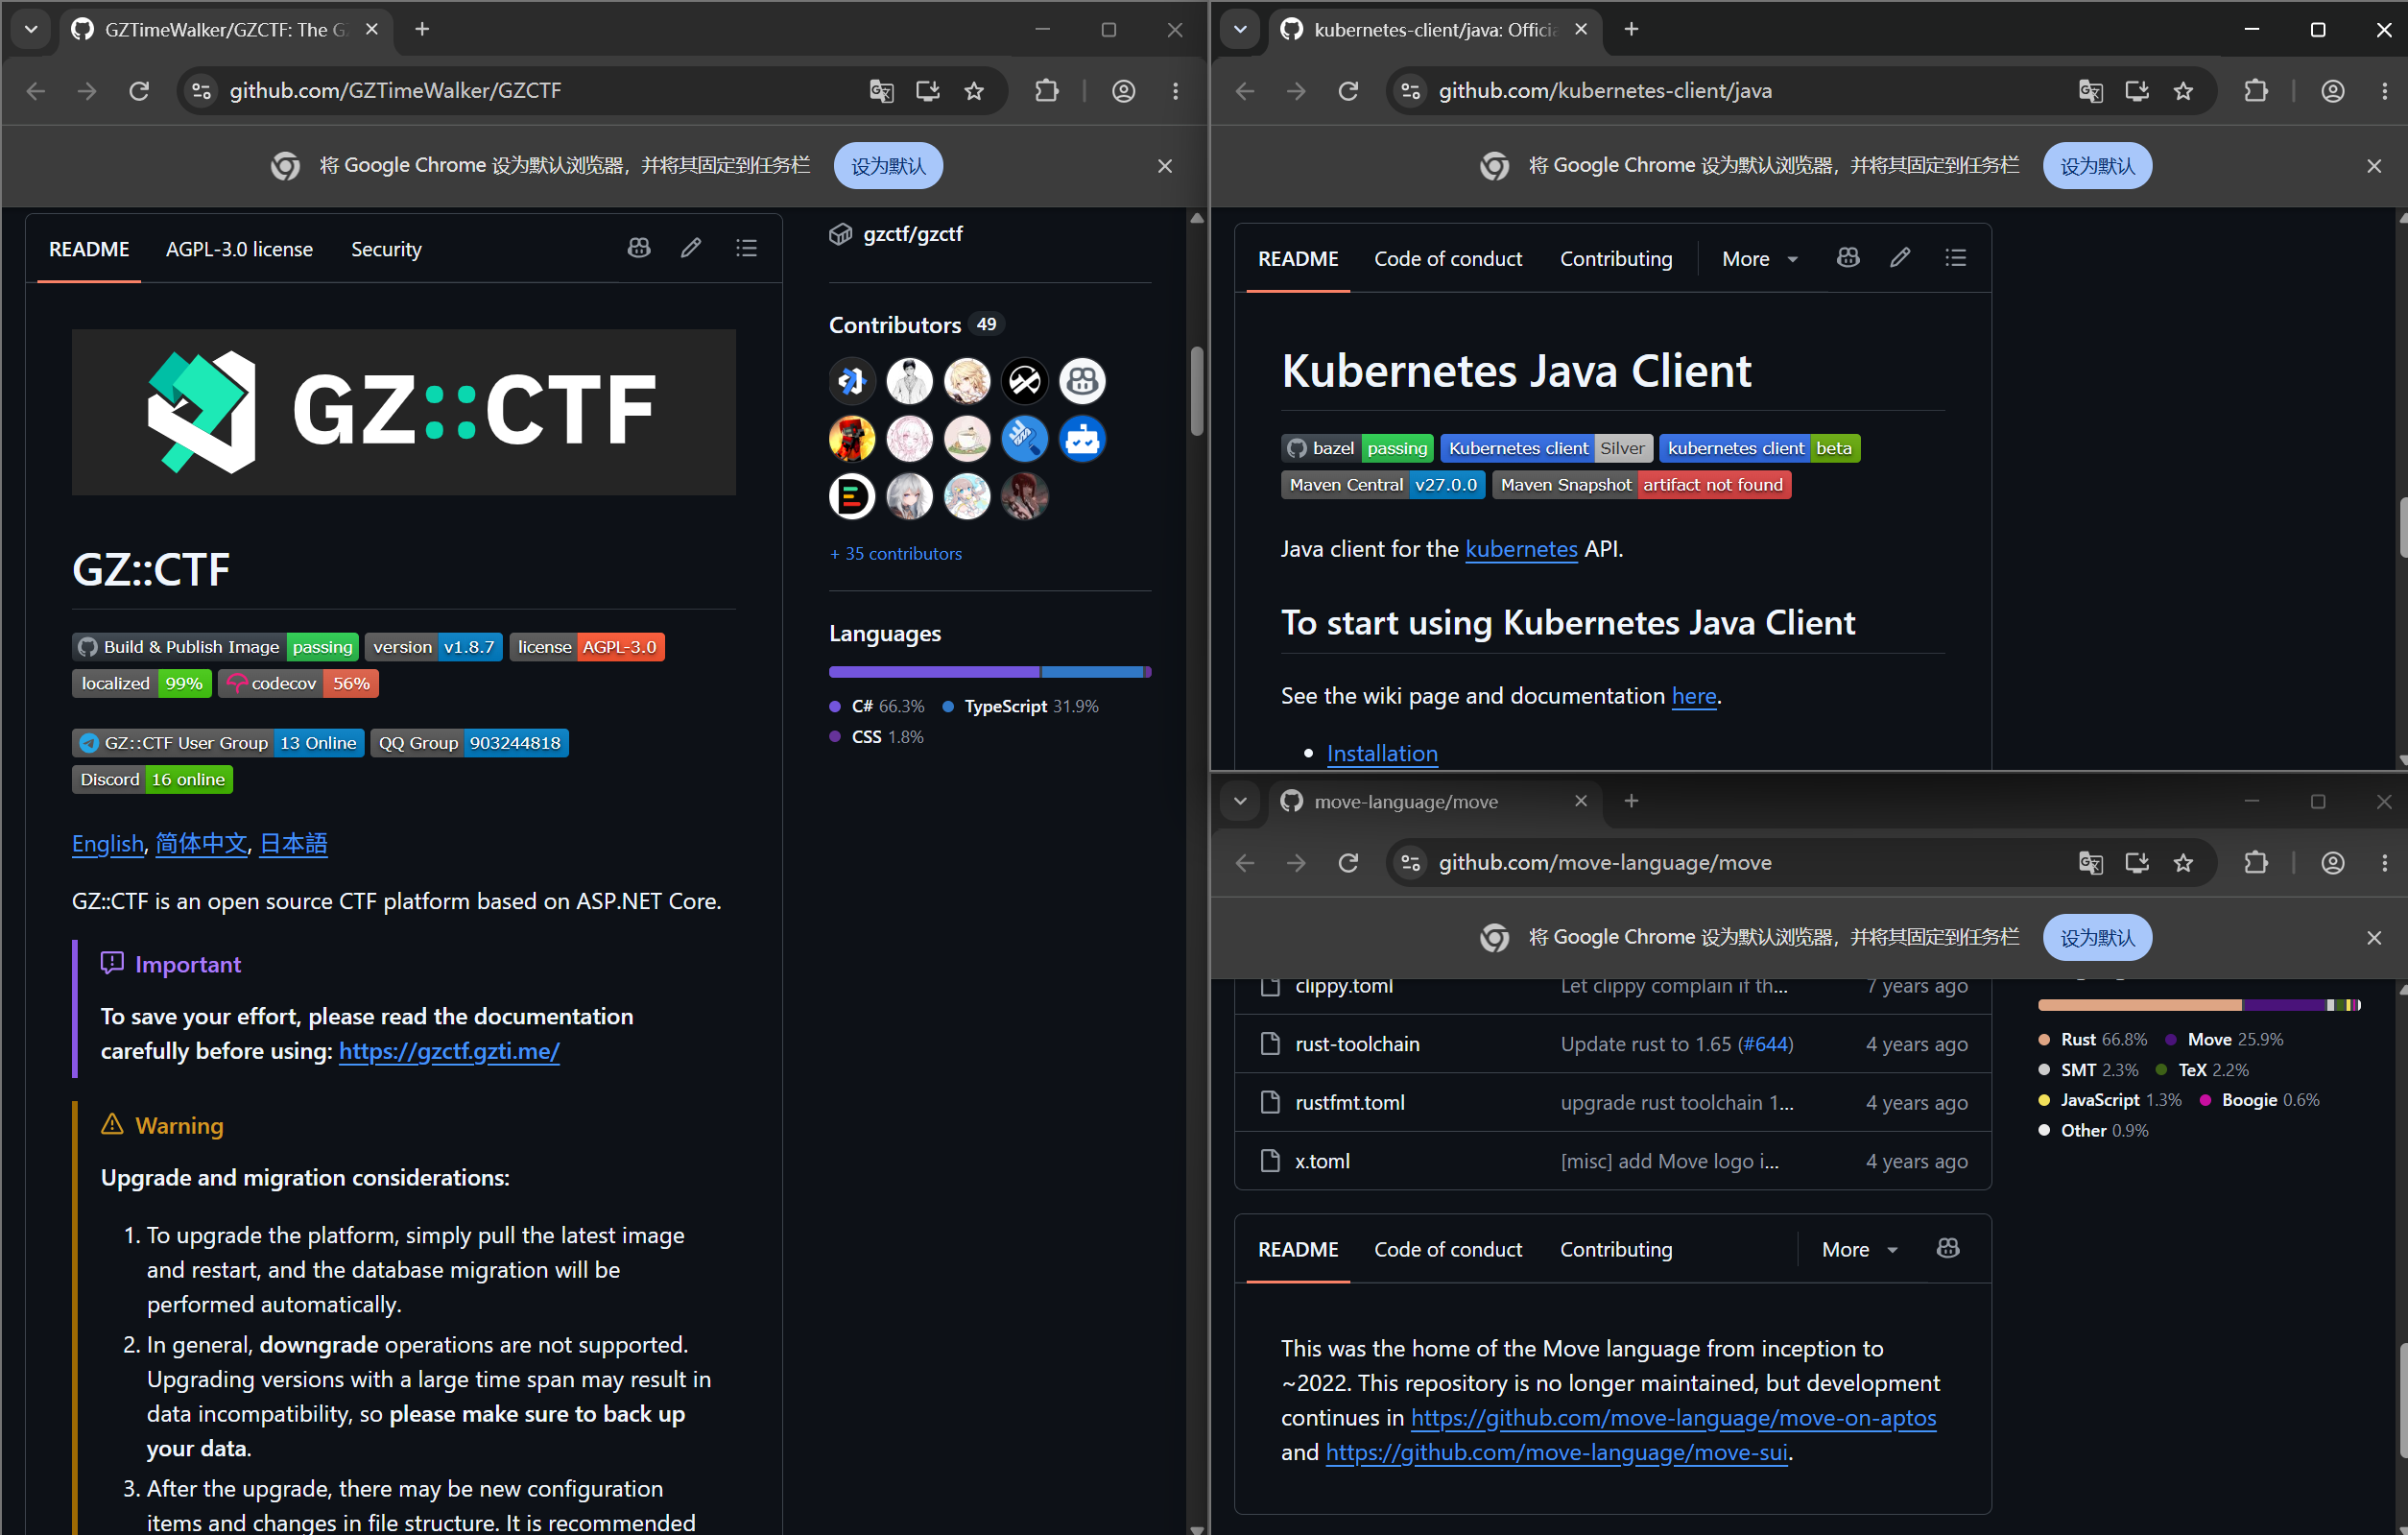
\includegraphics[width=\textwidth]{work03-6.png}
        \caption{三个仓库的 README} 
        \label{work03-6}
      \end{figure}
    \subsection{第07题}
      \subsubsection{题目描述}
      用 AI 编程智能体浏览一个陌生的代码库。最好在调试或为你在意的项目添加新功能的背景下进行。如果想不出合适的，可以试试用 AI 智能体理解 opencode 中安全相关功能的工作原理。
      \subsubsection{解题过程}
      将 opencode 的仓库 git clone 到本地，将项目交给 Trae 打开，给定提示词和约束“现在打开的项目是 opencode 的github 仓库，请查看仓库尝试总结 opencode 中安全相关功能的工作原理。要求：不能修改项目和其他文件。”。经过分析后 Agent 认为 opencode 采用“本机可信代理”模型——工具以宿主用户的完整文件/进程/网络权限运行，安全性由权限门控、路径边界、凭据保护、本地监听四层构成。AI完整回答见 github 仓库中 week03/ai\_summary.md。
      \noindent
      \begin{figure}[H]
        \centering
        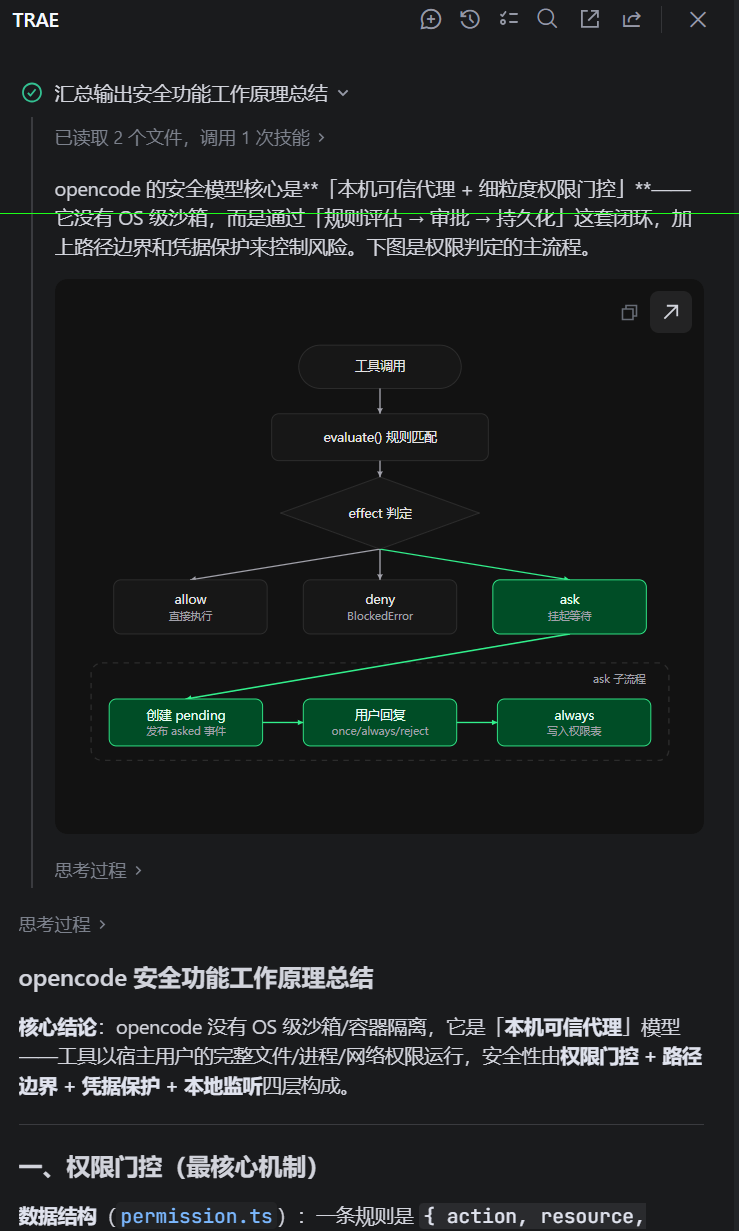
\includegraphics[width=\textwidth]{work03-7.png}
        \caption{智能体回答部分截图} 
        \label{work03-7}
      \end{figure}
    \subsection{第08题}
      \subsubsection{题目描述}
      编写一个函数 make\_counter()，它返回一个内部函数。每次调用该内部函数时，计数器加一并返回当前值。要求使用闭包实现，并解释为什么需要使用 nonlocal 关键字。
      \subsubsection{解题过程}
      在 python 中函数也是对象，因此可以在函数中定义函数并返回一个函数作为其值。需要注意的是函数中的嵌套函数使用的来自外层函数的变量则出现闭包现象，此时由于这个变量并非内层函数的局部变量，需要在内部函数使用 nonlocal 关键字进行声明。多次调用 make\_counter 所生成的函数对象是独立的，数据互不干扰。
      \noindent
      \begin{figure}[H]
        \centering
        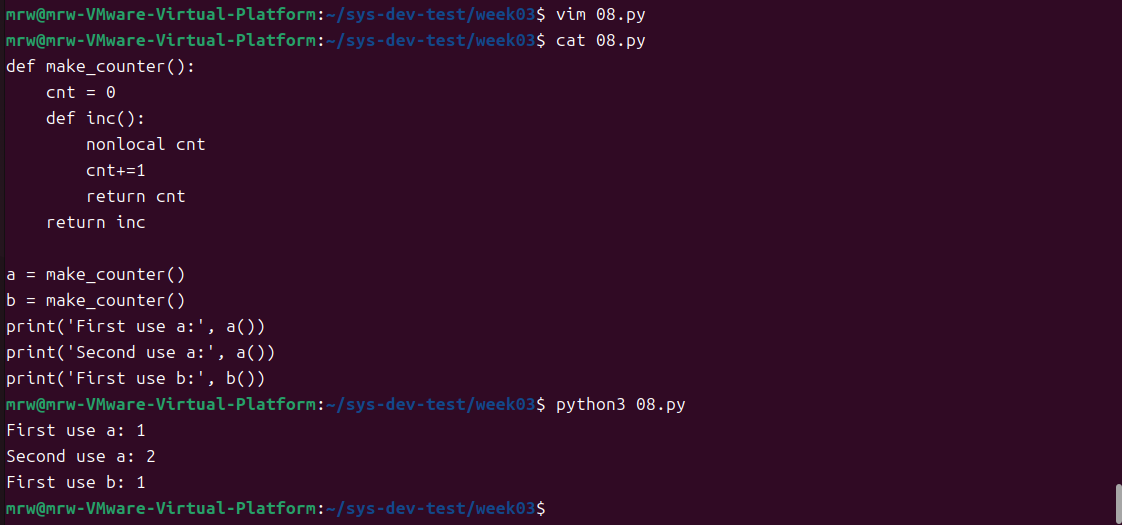
\includegraphics[width=\textwidth]{work03-8.png}
        \caption{python 函数闭包的实现} 
        \label{work03-8}
      \end{figure}
    \subsection{第09题}
      \subsubsection{题目描述}
      编写一个函数 append\_to(element, target=[])，将 element 追加到 target 并返回 target。不传 target 调用两次。解释输出并用 None 作为默认值修复该函数。
      \subsubsection{解题过程}
      直接编写函数，发现第二次调用时输出的是 [1,2] 而非 [2] 。这是因为 python 的函数对象的默认参数值若为列表，这个列表只会创建1次，导致后续调用时修改的是同一个列表。解决方案是默认传参为 None，若检测到 target 值为 None 则新建列表作为 target。
      \noindent
      \begin{figure}[H]
        \centering
        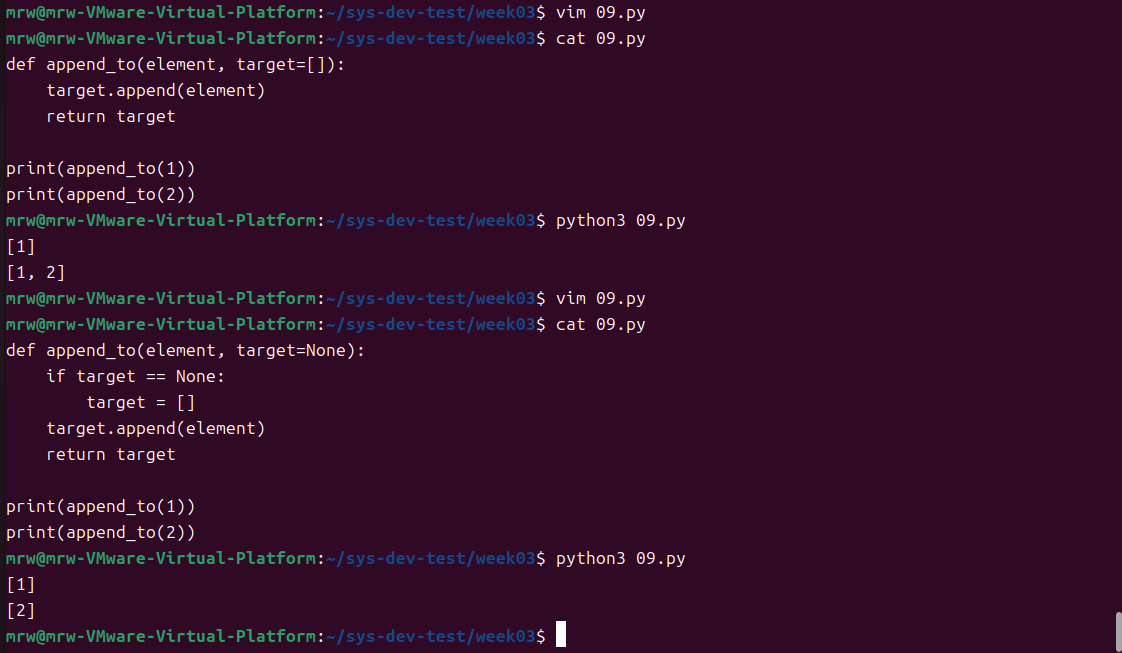
\includegraphics[width=\textwidth]{work03-9.png}
        \caption{默认参数陷阱及解决方案} 
        \label{work03-9}
      \end{figure}
    \subsection{第10题}
      \subsubsection{题目描述}
      给定 a = [[1, 2], [3, 4]]，创建 b = a.copy() 和 c = copy.deepcopy(a)。修改 a[0][0] = 99。打印 a、b、c。解释原因。并解释 is 和 == 的区别，用小整数和列表举例。
      \subsubsection{解题过程}
      a.copy() 虽然创建了新列表，但执行浅拷贝，内部元素依旧应用自旧列表，导致两个列表的修改会相互影响。需要使用 copy.deepcopy(a) 才能进行深拷贝创建完全独立的列表。 is 运算符检查对象地址是否相同（值也必定相同），== 运算符只检查值是否相同。无论通过深拷贝还是浅拷贝，所创建的列表对象自身都使用不同的内存地址，故 is 始终为 False 。对于整数而言，小整数和其他相同的字面量可能会共享内存地址（小整数在 CPython 中被缓存，而相同的字面量会被放入常量池），从而导致 is 也为 True。
      \noindent
      \begin{figure}[H]
        \centering
        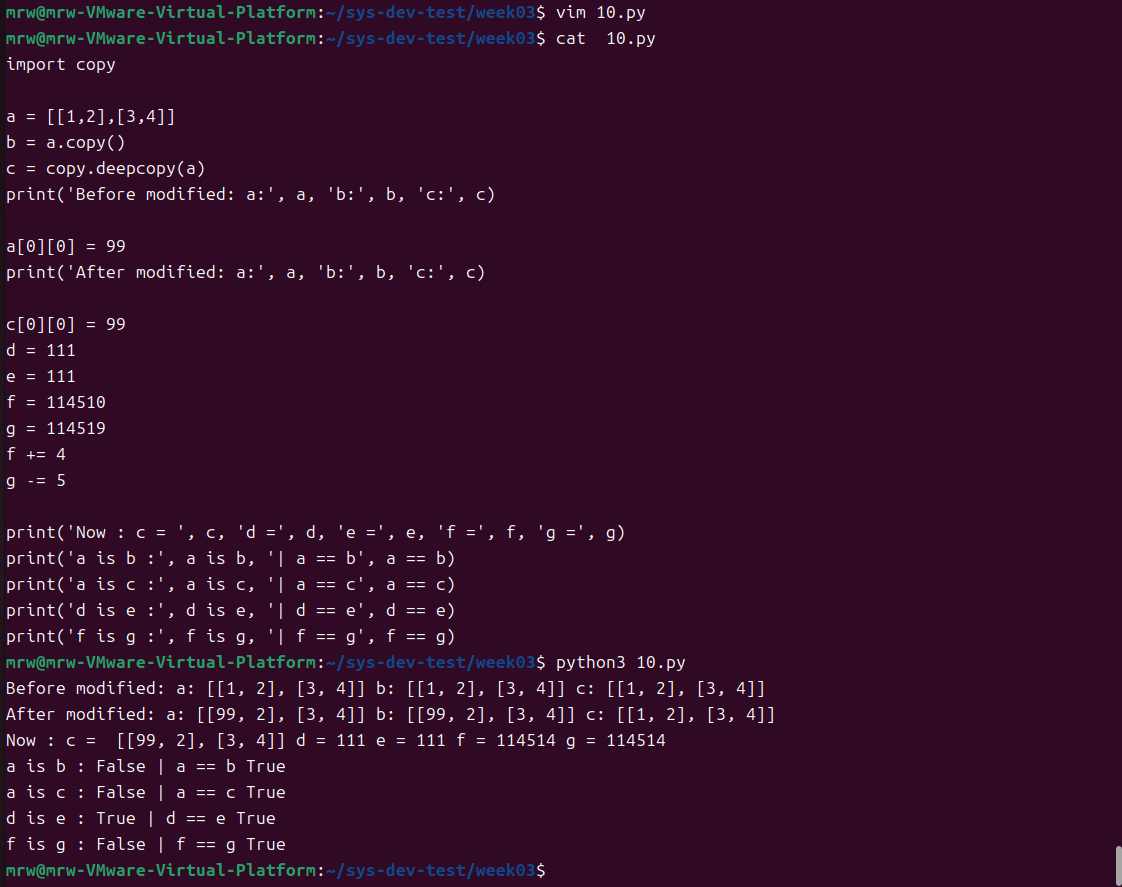
\includegraphics[width=\textwidth]{work03-10.png}
        \caption{深拷贝与浅拷贝以及 is 和 == 的演示} 
        \label{work03-10}
      \end{figure}
  \section{commit 记录}
  \noindent
  下面为对应的 commit 提交页面，具体提交详情见 github 仓库。
      \noindent
      \begin{figure}[H]
        \centering
        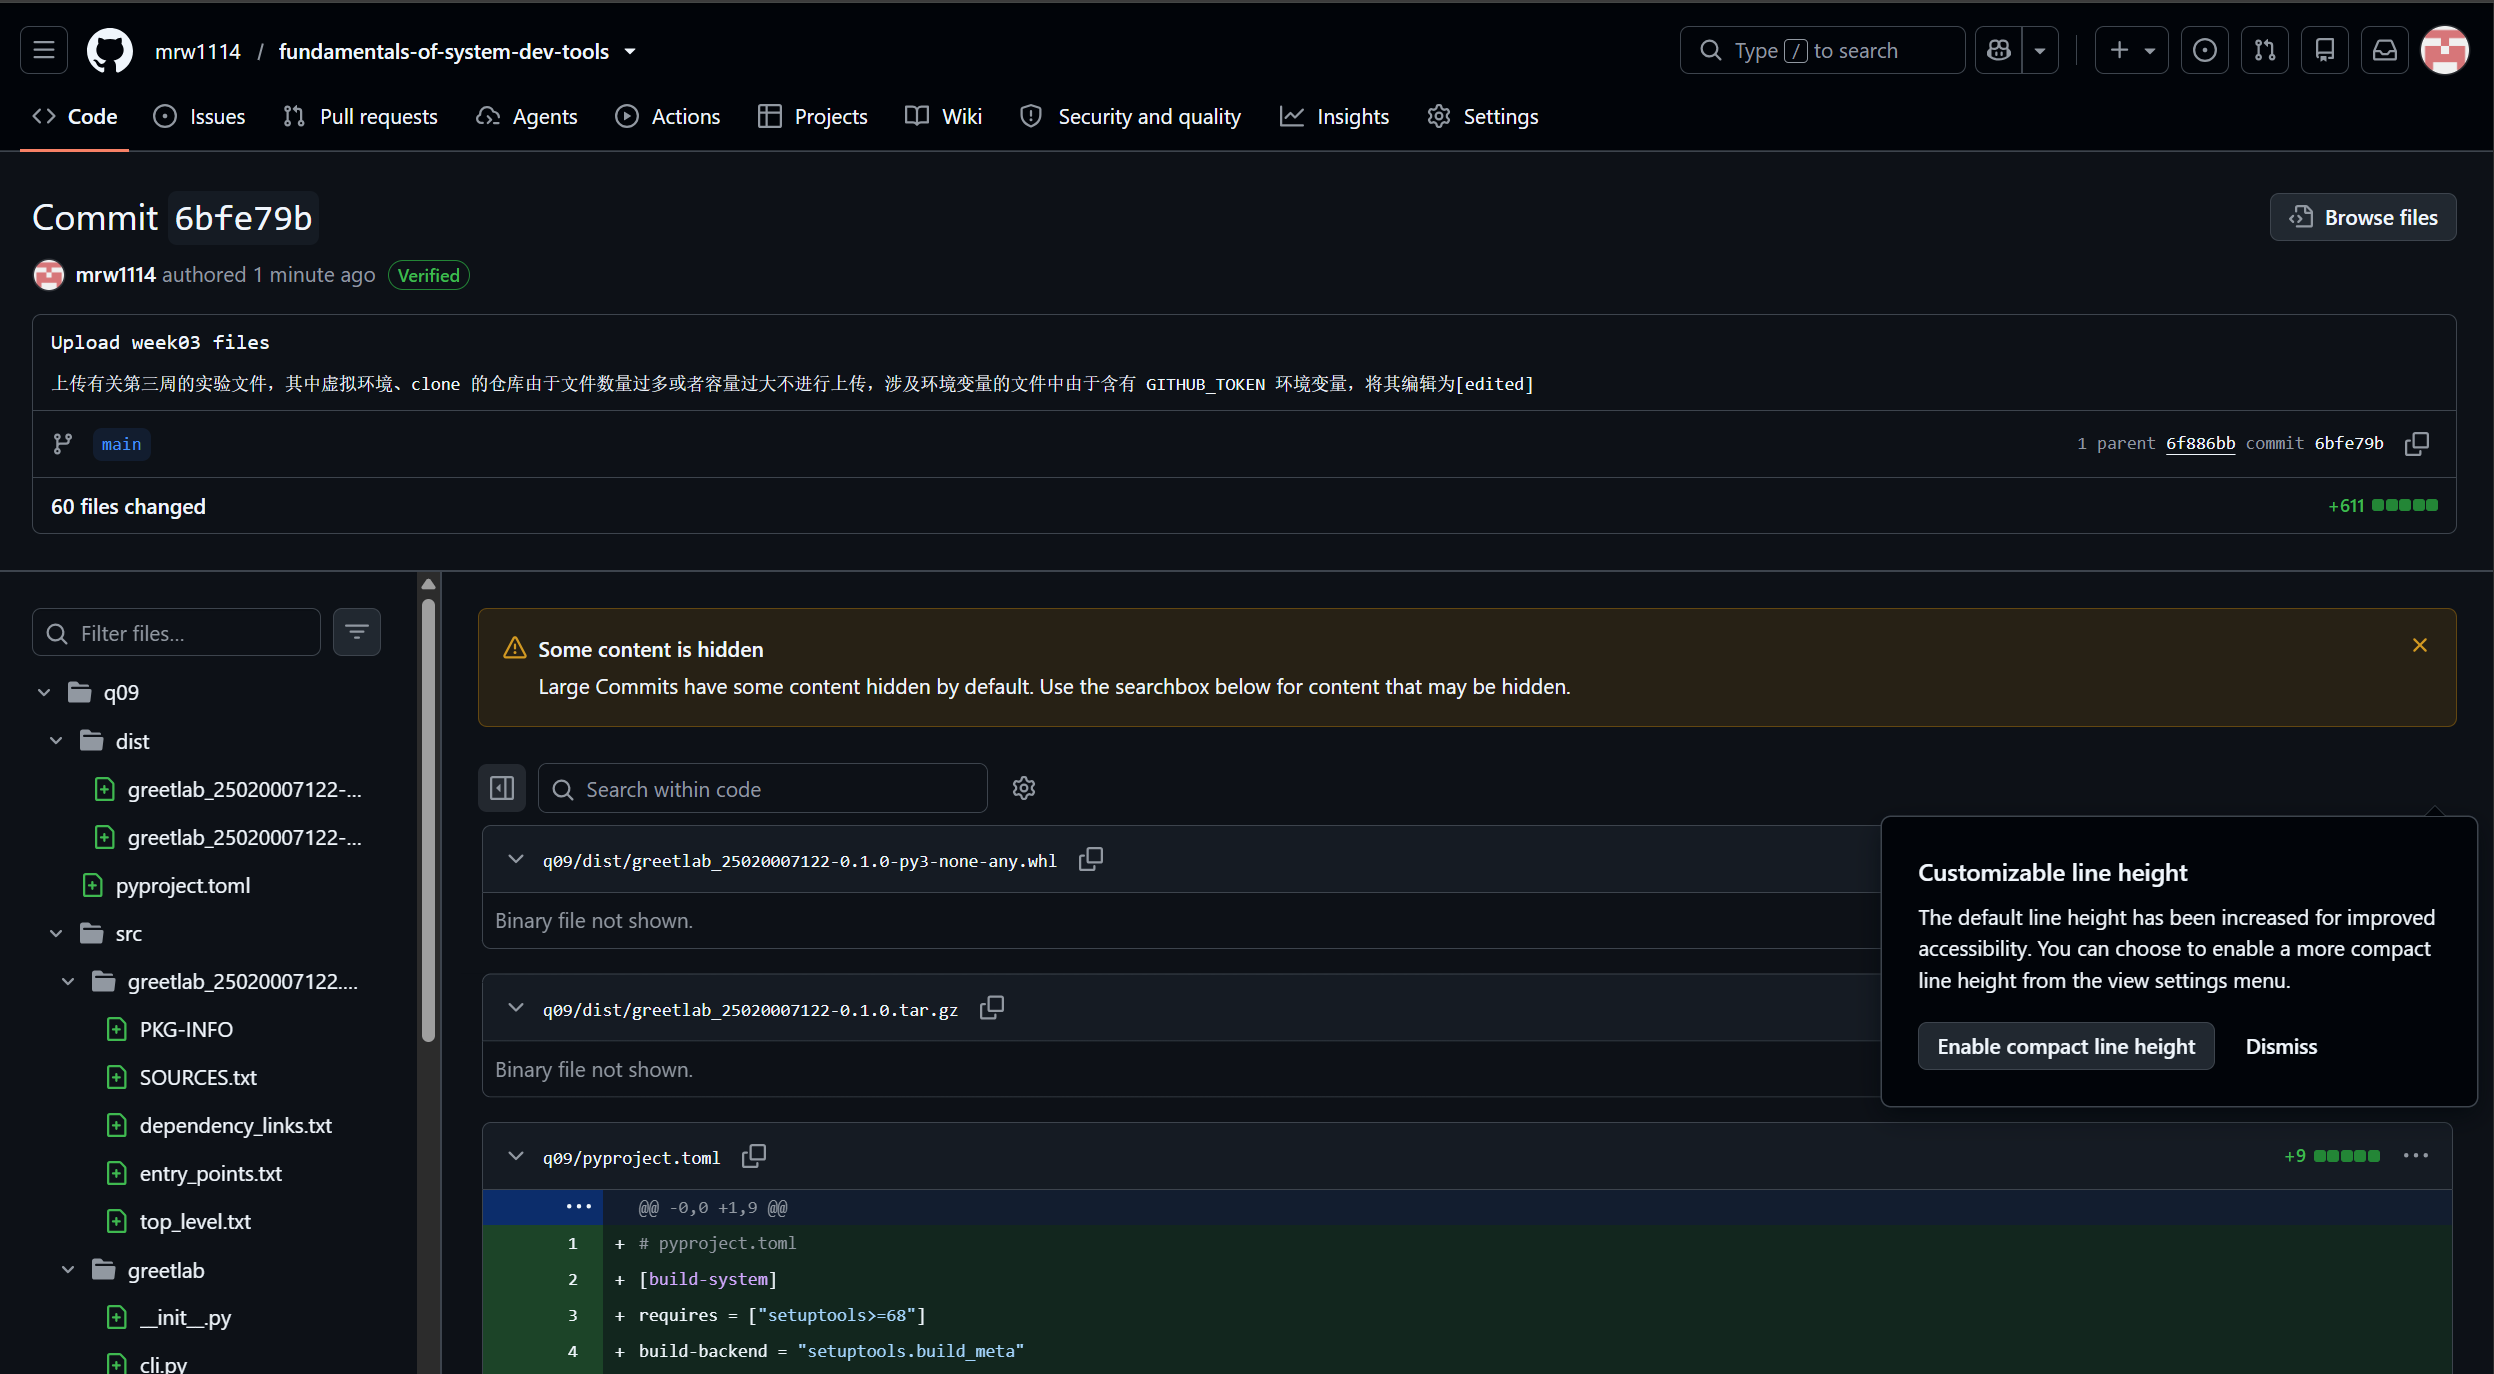
\includegraphics[width=\textwidth]{history3.png}
        \caption{提交历史记录}
        \label{history3}
      \end{figure}

\end{document}
